\makeatletter
\def\input@path{{../../}}
\makeatother
\documentclass[../../main.tex]{subfiles}

\graphicspath{
  {../../img/}
  {../img/}
  {img/}
}

\begin{document}
	\section{Необходимое условие ЛЭФНП}
	Рассмотрим ФНП $u = f (x)$,
	где $x = (x_1, \ldots, x_n) \in D \subset \R^n$.
	
	Внутрення точка $x_0 = (x_{0 1}, \ldots, x_{0n}) \in D$
	называется \emph{точкой строгого локального минимума (максимума)}
	$f(x)$,
	если
	\[
		\exists V (x_0) \subset D:
		\ \forall x \in \dot{V} (x_0)
		= V (x_0) \setminus \{x_0\}
		\implies f (x_0) < f (x)
		\quad \big(f (x) < f (x_0)\big).
	\]
	Если $\forall x \in V (x_0)$ мы можем гарантировать
	только нестрогие неравенства $f (x_0) \le f (x)
	\\ \displaystyle
	\big(f (x) \le f (x_0)\big)$,
	то $x_0$ называется просто \emph{точкой локального минимума (максимума)}.
	
	Общее название таких точек
	--- \emph{точки локального экстремума} для $f (x)$.
	
	Значение $f (x)$ в точке локального экстремума $x_0$
	соответственно будем обозначать
	$f_{min} = f (x_{min})$ и $f_{max} = f (x_{max})$
	и называть \emph{экстремальными значениями} ЛЭФНП.
	
	\begin{exmp}
		Рассмотрим Ф2П
		\[
		\begin{cases}
			u = f (x, y) = x^2 + y^2, \\
			\forall (x, y) \in \R^2. \\
		\end{cases}
		\]
		Для этой функции в пространстве $\R^3$ графиком $\Gamma_f$
		будет являться поверхность $z = x^2 + y^2$,
		соответствующая эллиптическому параболоиду в ДПСК $Oxyz$.
		\[
			\forall (x, y) \ne (0, 0)
			\implies
			f (x, y) = x^2 + y^2 > 0 = f (0, 0),
		\]
		поэтому точка $M_0 (0, 0) \in \R^2$
		будет являться точкой строгого локального минимума рассматриваемой Ф2П,
		при этом $f_{min} = f (M_0) = 0$.
		
		В данном случае
		этот минимум является не только локальным, но и глобальным.
		
		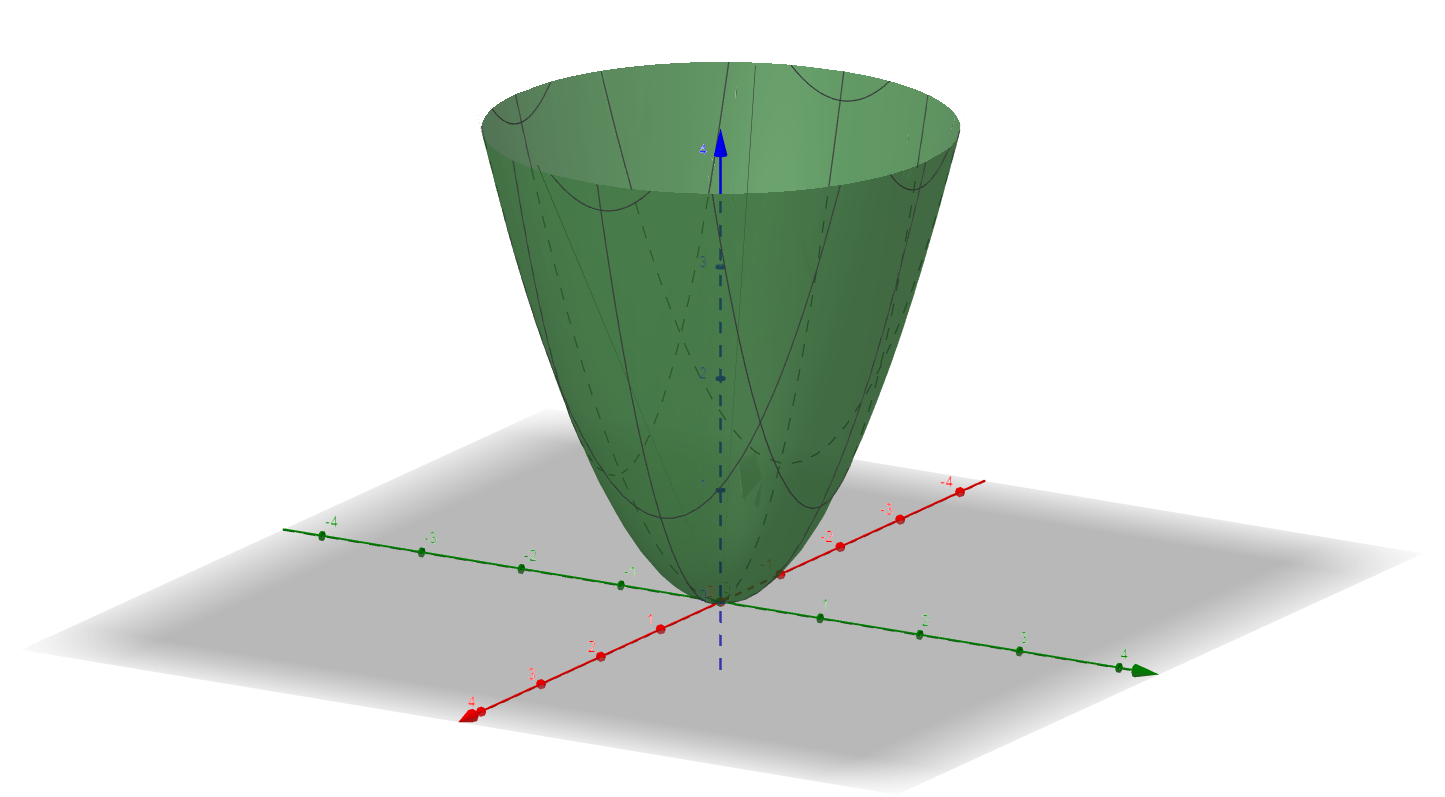
\includegraphics[width=0.9\linewidth]{Ellyptic_paraboloid}
		
	\end{exmp}
	
	Для определения локального экстремума на языке приращений,
	придадим внутренней точке $x_0 \in D$
	произвольные приращения $\D x \in \R^n$ так,
	чтобы $(x_0 + \D x) \in D$.
	Тогда, учитывая, что $\D f (x_0)
	= f (x_0 + \D x) - f (x_0)$,
	в случае, когда $x_0 = x_{min}$, получим
	$f (x_0 + \D x) - f (x_0) \ge 0
	\implies
	\D f (f_0) \ge 0$.
	Аналогично, если $x_0 = x_{max}$,
	то тогда $\D f (x_0) \le 0$.

	Таким образом, $x_0$ --- точка локального экстремума ФНП
	тогда и только тогда, когда
	приращение функции $\D f (x_0)$ на допустимом
	произвольном $\D x \in \R^n$ сохраняет один и тот же знак.
	
	В случае, когда для допустимых произвольных $\D x \ne 0 \implies
	\D f (x_0) > 0 \displaystyle
	\quad \big(\D f (x_0) < 0\big)$
	имеем в $x_0$ строгий локальный минимум (максимум).
	
	\begin{thm}[Необходимое условие ЛЭФНП]
		Пусть ФНП
		\[
		\begin{cases}
			u = f (x), \\
			x = (x_1, \ldots, x_n) \in D \subset \R^n; \\
		\end{cases}
		\]
		дифференцируема в некоторой окрестности $V (x_0) \subset D$
		внутренней точки $x_0 \in D$. Если эта $x_0$ является экстремальной
		для $f (x)$, то $x_0$ --- стационарная точка
		для $f (x)$, т.е. для произвольных допустимых
		\begin{equation}
		\label{nec cond loc extr}
			\forall dx = \D x \in \R^n \implies df (x_0) = 0.
		\end{equation}
	\end{thm}
	\begin{proof}
		Придавая точке $x_0 \in V (x_0) \subset D$
		произвольное приращение \\
		$\D x = (\D x_1, \ldots, \D x_n) \in \R^n$ так,
		чтобы $(x_0 + \D x) \in V (x_0)$,
		наряду с общим приращением функции
		$\D f (x_0) = f (x_0 + \D x) - f (x_0)$,
		рассмотрим для фиксированного $k = \overline{1, n}$
		соответствующее специальное приращение
		$\D_k x = \left(0, \ldots, 0,
		\underbrace{\D x_k}_{k\text{-е место}}, 0, \ldots, 0\right)$,
		для которого
		$(x_0 + \D_k x)
		= \left(x_{0 1}, \ldots, x_{0, k - 1}, x_{0 k} + \D x_k,
		x_{0, k + 1}, \ldots, x_{0 n}\right) \in V (x_0)$.
		
		В результате получим соответствующие специальные приращения
		рассматриваемой функции по $k$-й координате
		$\D_k f (x_0)
		= f (x_0 + \D_k x) - f (x_0)$.
		Если $x_0$ --- точка локального минимума (максимума)
		для $f (x)$, то $\D f (x_0) \ge 0
		\displaystyle
		\quad \big(\D f (x_0) \le 0\big)$,
		откуда следует, что $\D_k f (x_0) \ge 0
		\displaystyle
		\quad \big(\D_k f (x_0) \le 0\big)$,
		т.е. точка $t_k = x_{0 k}$ будет точкой локального минимума (максимума)
		Ф1П $F_k (t)
		= f (x_{0 1}, \ldots, x_{0, k - 1}, t,
		x_{0, k+1}, \ldots, x_{0 n})$,
		так как здесь 
		\[
			\D F_k (t_k)
			= F_k (x_{0 k} + \D t) - F (x_{0 k})
			= \D_k f (x_0) \ge 0.
		\]
		Используя далее необходимое условие локального экстремума Ф1П получим,
		что точка $t_k = x_{0 k}$ является для $F_k (t)$
		стационарной, т.е. 
		\[
			F'_k (t_k) = 0.
		\]
		Отсюда, учитывая, что 
		\[
			F'_k (t_k)
		= \pderiv{f (x_0)}{x_k},\ k = \overline{1, n},
		\]
		имеем
		\[
			df (x_0)
			= \sum_{k = 1}^{n}
			\underbrace{\pderiv{f (x_0)}{x_k}}_{= 0} dx_k
			= 0. \qedhere
		\]
	\end{proof}
	\begin{rem}
		Как и для Ф1П, условие \eqref{nec cond loc extr} в общем случае
		лишь необходимо для экстремальности $x_0$, так как не всякая
		стационарная точка может быть экстремальной. \\
		Например, для Ф2П
		\[
		\begin{cases}
			u = f (x, y) = x^2 - y^2, \\
			(x, y) \in \R^2; \\
		\end{cases}
		\]
		из системы
		\[
		\begin{cases}
			f'_x = 2x = 0, \\
			f'_y = 2y = 0; \\
		\end{cases}
		\]
		получим, что точка $M_0 (0, 0)$ --- стационарная,
		$df (M_0) = 0$,
		но здесь она не будет экстремальной, так как на специальных приращениях
		$(\D x, \D y) \in \R^2$ имеем
		\begin{enumerate}
			\item[а)]
			если
			\[
			\begin{cases}
				\D x = 0, \\
				\D y \ne 0; \\
			\end{cases},
			\]
			то
			\[
				\D f (M_0)
				= f (0, \D y) - f (0, 0)
				= -y^2 < 0;
			\]
			
			\item[б)]
			\[
			\begin{cases}
				\D x \ne 0, \\
				\D y = 0; \\
			\end{cases}
			\implies
			\D f (M_0)
			= x^2 > 0.
			\]
		\end{enumerate}
		Значит, $\forall V (M_0) \subset \R^2$ (приращение функции)
		не сохраняет один и тот же знак, т. е. стационарная точка $M_0$
		не будет экстремальной.
	\end{rem}
	
	\section{Квадратичные формы (КФ) и некоторые их свойства}
	В дальнейшем, для получения достаточных условий экстремальности
	стационарных точек ФНП нам понадобятся соответствующие свойства КФ,
	т.е. форм от $n$ переменных $h = (h_1, \ldots, h_n) \in \R^n$ вида
	\begin{equation}
	\label{quad form}
		\Phi(h) = \sum_{i, j = 1}^n a_{i j} h_i h_j,
		\quad \forall a_{i j} \in \R,\ i = \overline{1, n},\ j = \overline{1, n}.
	\end{equation}
	Для \eqref{quad form} матрица
	\begin{equation}
	\label{form matrix}
		A =
		\begin{bmatrix}
			a_{1 1} & a_{1 2} & \ldots & a_{1 n} \\
			a_{2 1} & a_{2 2} & \ldots & a_{2 n} \\
			\vdots & \vdots & \ddots & \vdots \\
			a_{n 1} & a_{n 2} & \ldots & a_{n n} \\
		\end{bmatrix}
		\text{ ---}
	\end{equation}
	матрица квадратичной формы \eqref{quad form}.
	
	\begin{exmp}
		Для $n = 3$ имеем $\Phi(h_1, h_2, h_3) \stk{quad form}{=} \ldots
		= a_{1 1} h_1^2 + a_{2 2} h_2^2 + a_{3 3} h_3^2
		+ (a_{1 2} + a_{2 1}) h_1 h_2 + (a_{1 3} + a_{3 1}) h_1 h_3
		+ (a_{2 3} + a_{3 2}) h_2 h_3$.
		Квадратичная форма будет иметь матрицу
		\[
			A =
			\begin{bmatrix}
				a_{1 1} & a_{1 2} & a_{1 3} \\
				a_{2 1} & a_{2 2} & a_{2 3} \\
				a_{3 1} & a_{3 2} & a_{3 3} \\
			\end{bmatrix}.
		\]
	\end{exmp}
	В общем случае, для матриц \eqref{form matrix} квадратичных форм
	\eqref{quad form} её \emph{главными угловыми минорами} называют
	определители
	\begin{equation}
	\label{main corner minors}
	\begin{array}{c}
		\D_1 = a_{1 1}, \\ \\
		\D_2 =
		\begin{vmatrix}
			a_{1 1} & a_{1 2} \\
			a_{2 1} & a_{2 2} \\
		\end{vmatrix}, \\ \\
		\D_3 =
		\begin{vmatrix}
			a_{1 1} & a_{1 2} & a_{1 3} \\
			a_{2 1} & a_{2 2} & a_{2 3} \\
			a_{3 1} & a_{3 2} & a_{3 3} \\
		\end{vmatrix}, \\
		\dots \\
		\D_n = \det A.
    \end{array}
	\end{equation}
	
	Нетрудно видеть, что на тривиальном наборе
	$\vec{0} = (0, \ldots, 0) \in \R^n$ любая КФ \eqref{quad form}
	даёт $\Phi(\vec{0}) \stk{quad form}{=} 0$.
	
	В дальнейшем, КФ \eqref{quad form} будем называть \emph{неположительной
	(неотрицательной)}, если $\forall h \in \R^n \implies
	\Phi(h) \ge 0
	\quad \big(\Phi(h) \le 0\big)$.
	
	КФ \eqref{quad form} называют \emph{положительно (отрицательно) определённой}
	или \emph{знакоположительной (знакоотрицательной)},
	если $\forall h \ne \vec{0} \implies \Phi(h) > 0 \quad \big(\Phi(h) < 0\big)$.
	Общее название таких КФ --- знакопостоянные (знакоопределённые) КФ.
	
	КФ \eqref{quad form} называют \emph{вырожденной}, если
	$\exists h_0 \ne \vec{0} \implies \Phi(h_0) = 0$.
	Вырожденные КФ \eqref{quad form}, для которых
	$\forall h \in \R^n \implies \Phi(h) \ge 0
	\quad \big(\Phi(h) \le 0\big)$,
	называют \emph{полуопределёнными}.
	
	На практике, как правило, будем рассматривать симметрические КФ
	\eqref{quad form}, т.е. у которых матрица \eqref{form matrix} симметрическая
	$\left(A^T = A \iff a_{i j} = a_{j i},
	\forall i = \overline{1, n},\ \forall j = \overline{1, n}\right)$.
	Например, симметрическая матрица 3-го порядка
	\[
		A =
		\begin{bmatrix}
			a_{1 1} & a_{1 2} & a_{1 3} \\
			a_{1 2} & a_{2 2} & a_{2 3} \\
			a_{1 3} & a_{2 3} & a_{3 3} \\
		\end{bmatrix}
	\]
	соответствует КФ
	\[
		\Phi(h_1, h_2, h_3)
		= a_{1 1} h_1^2 + a_{2 2} h_2^2 + a_{3 3} h_3^2
		+ 2 a_{1 2} h_1 h_2 + 2 a_{1 3} h_1 h_3 + 2 a_{2 3} h_2 h_3
	\]
	и наоборот.
	
	Имеет место \emph{критерий Сильвестра знакоопределённости КФ}:
	\begin{enumerate}
		\item
		симметрическая КФ \eqref{quad form} является знакоположительной
		(положительно определённой)
		тогда и только тогда, когда
		все главные угловые миноры \eqref{main corner minors} её матрицы
		положительны,
		т.е. $\forall \D_k > 0, k = \overline{1, n}$;
		
		\item
		для того, чтобы симметрическая КФ \eqref{quad form}
		была знакоотрицательной, необходимо и достаточно, чтобы все главные
		угловые миноры \eqref{main corner minors} имели знакочередующиеся
		значения, а именно: $\D_1 < 0, \D_2 > 0, \D_3 < 0,
		\ldots, (-1)^n \D_n > 0$.
	\end{enumerate}
	
	Исследование симметрической КФ \eqref{quad form} на знакоопределённость
	можно проводить методом Лагранжа выделения полных квадратов.
	
	\begin{exmp}
		Пусть
		\[
			\Phi(h_1, h_2, h_3)
			= 2 h_1^2 + 3 h_2^2 + h_3^2 - 4 h_1 h_2 + 2 h_1 h_3 - 2 h_2 h_3.
		\]
		Её матрицей будет
		\[
			A =
			\begin{bmatrix}
				2 & -2 & 1 \\
				-2 & 3 & -1 \\
				1 & -1 & 1 \\
			\end{bmatrix}.
		\]
		\begin{description}
			\item[I способ (по критерию Сильвестра):]
			имеем $\D_1 = 2 > 0,\ \D_2 =
			\begin{vmatrix}
				2 & -2 \\
				-2 & 3 \\
			\end{vmatrix}
			= 2 > 0, \\
			\D_3 = \det A = \ldots = 1 > 0$,
			поэтому рассматриваемая матрица, а, значит, и соответствующая ей КФ,
			положительно определена (знакоположительна);
			
			\item[II способ (метод Лагранжа выделения полных квадратов):]
			будем выделять последовательно полные квадраты с переменной $h_3$:
			\begin{gather*}
				\Phi
				= (h_3^2 + 2(h_1 - h_2) h_3) + 2 h_1^2 + 3 h_2^2 - 4 h_1 h_2
				= \\ = \left[\dfrac{1}{2}\cdot \pderiv{\Phi}{h_3}
				= h_3 + h_1 - h_2\right]
				= (h_3 + h_1 - h_2)^2 - (h_1 - h_2)^2 + 2 h_1^2 + 3 h_2^2
				- 4 h_1 h_2
				= \\ = (h_3 + h_1 - h_2)^2 + \underbrace{h_1^2 - 2 h_1 h_2
				+ 2 h_2^2}_{\Phi_0}
				= \left[\dfrac{1}{2} \pderiv{\Phi_0}{h_1}
				= h_1 - h_2\right]
				= \\ = (h_3 + h_1 - h_2)^2 + (h_1 - h_2)^2 + h_2^2 \ge 0.
			\end{gather*}
			Значит, рассматриваемая КФ неотрицательна.
			Осталось показать, что она невырождена,
			т.е. только на наборе $h_0 = (0, 0, 0) \implies
			\Phi(h_0) = 0$:
			\begin{gather*}
				\Phi(h = 0)
				\iff
				\begin{cases}
					h_3 + h_1 - h_2 = 0, \\
					h_1 - h_2 = 0, \\
					h_2^2 = 0; \\
				\end{cases}
				\iff
				h_1 = h_2 = h_3 = 0.
			\end{gather*}
			Поэтому рассматриваемая КФ невырождена, неотрицательна,
			а, значит, положительно определена.
		\end{description}
	\end{exmp}
	
	В дальнейшем нам понадобится вспомогательная
	\begin{lem}[Оценка знакопостоянной КФ]
		Если КФ \eqref{quad form} является знакопостоянной, то
		\begin{equation}
		\label{eval form}
			\exists C_0 = const > 0,\ 
			\forall h \in \R^n,\ \abs{h} = \sqrt{h_1^2 + \ldots + h_n^2} = 1
			\implies \Phi(h) \ge C_0.
		\end{equation}
	\end{lem}
	\begin{proof}
		Во-первых, множество $h \in \R^n$, для которых $\abs{h} = 1$,
		представляет собой $n$-мерную единичную сферу $S = S_1(\vec{0})$
		радиуса $R = 1$ с центром в начале координат
		$\vec{0} = (0, \ldots, 0) \in \R^n$.
		
		Эта сфера является ограниченным замкнутым множеством в $\R^n$, т.е.
		компактом, поэтому, в силу непрерывности функции $\abs{\Phi(h)}$
		на компакте $S \subset \R^n$, по теореме Вейерштрасса, получили
		достижимость, например, минимального значения на $S$, т.е.
		\[
			\exists h_0 \in S \implies
			C_0 = \min_{h \in S} \abs{\Phi(h)}
			= \abs{\Phi(h_0)} \ge 0.
		\]
		В данном случае, так как $h_0 \in S$, то
		$\abs{h_0} = 1 \implies h_0 \ne \vec{0} \in \R^n$,
		поэтому, в силу знакопостоянства рассматриваемой КФ
		получили её невырожденность, \\
		а поэтому $\Phi(h_0) \ne 0 \implies C_0 = \abs{\Phi(h_0)} > 0$.
	\end{proof}
\end{document}
